\chapter{Phonon Density of States}\label{ch:in4}

In this chapter, we take a closer look at the so-called phonon Density-of-States (DOS) in a series of insulating and superconducting samples with different dopant species. In the previous chapter, we looked at certain low-energy phonon branches which could be properly separated and measured due to the sparse nature of bands from \SIrange{0}{10}{\milli\eV}. This was due to the fact that the neutron differential cross-section `sees' preferentially vibrations parallel to the neutron wave vector due to the $\bm{Q} \cdot \bm{e}_j$ factor in equation \eqref{eq:one_phonon_sqw}. At higher energies, the phonon bands are heavily entangled (in the literal sense) making it difficult to separate different contributions to a measured spectrum where we have a finite resolution.

\begin{figure}
    \centering
    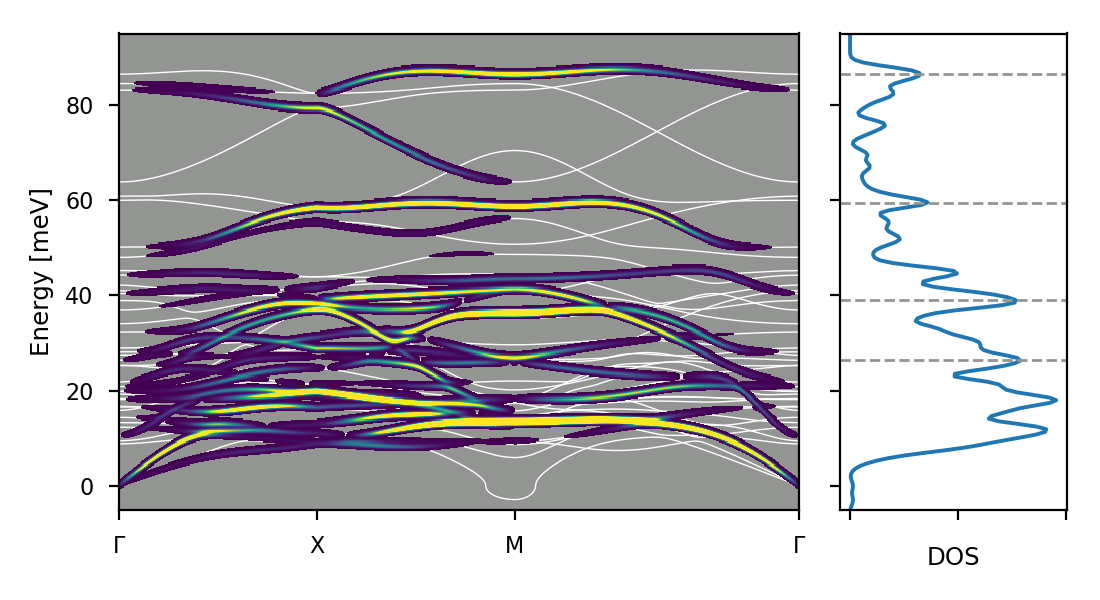
\includegraphics[width=0.8\textwidth]{fig/gdos/neutron_bands_dos_lto_afm.png}
    \caption{Neutron weighted phonon bands and DOS computed for La$_2$CuO$_4$ in the orthorhombic (LTO) crystal structure and magnetic, insulating electronic structure. \textbf{Left}: Band structure shown with neutron intensity where the energy axis have been given a Gaussian width of \SI{0.3}{\milli\eV} Full-Width Half-Maximum (FWHM). The white lines shows the $\delta$-function dispersion and thus reveal certain bands invisible to neutrons. \textbf{Right}: Phonon DOS obtained by integration of the first Brillouin Zone on a $20 \times 20 \times 20$ grid and broadening the spectra with a Gaussian width of \SI{1}{\milli\eV} FWHM. Certain Features that we observe in experiments are marked with grey horizontal lines. See discussion in the text, figure \ref{fig:gdos_10k} and table \ref{tab:gdos_features_10K}.}
    \label{fig:neutron_bands_dos_lto_afm}
\end{figure}

As a reminder, figure \ref{fig:neutron_bands_dos_lto_afm} shows the neutron-weighted bands in La$_2$CuO$_4$ with orthorhombic symmetry. At energies from \SIrange{10}{40}{\milli\eV} we have a lot of intensity originating from multiple bands. Even if we took the data in all these directions, which would be a very laborious task, comparing experiment and simulation would be much harder compared to the analysis performed in chapter \ref{ch:lowen}. On the right-hand side of figure \ref{fig:neutron_bands_dos_lto_afm} we see the neutron-weighted DOS, which is found by essentially summing up the three dimensional band structure onto the energy axis.

The advantage of using the phonon DOS, is that we can obtain a `dynamical fingerprint' of a specific sample and consequently compare different samples, temperatures or other parameters of interest. In addition, the phonon DOS can be obtained experimentally by measuring powders with a Time-of-Flight (ToF) spectrometer as we covered in section \ref{sec:specific_neutron}, chapter \ref{ch:method}.

\section{Experiment}
We performed inelastic neutron time-of-flight experiments on a series of La$_{2-x}$Sr$_{x}$CuO$_{4+\delta}$ powdered samples in order to better understand the relationship between mobile (O) and static (Sr) dopants similar to the objectives outlined for Pair-Distribution Function analysis in chapter \ref{ch:local}. The samples used here are listed in table \ref{tab:in4_samples} and are identical to the ones as used in \ref{ch:local}\todo{citation for Mariams thesis}. The naming scheme of table \ref{tab:in4_samples} will be used throughout this chapter.

\begin{table}
    \caption{Samples used in the experiment, along with a naming scheme used in this chapter, the composition and the superconducting transition temperature as obtained from susceptibility measurements. For additional details about these powdered samples see the thesis by M. Ahmad [XX].}
    \label{tab:in4_samples}
    \centering
    \begin{tabular}{lll}
    \toprule
      Name &                             Composition &                $T_\text{c}$ \\
    \midrule
       LCO &                           La$_2$CuO$_4$ &                           - \\
      LCOO &                      La$_2$CuO$_{4.05}$ &  $\approx \SI{40}{\kelvin}$ \\
     LSCO3 &           La$_{1.97}$Sr$_{0.03}$CuO$_4$ &                           - \\
     LSCO3 &  La$_{1.97}$Sr$_{0.03}$CuO$_{4+\delta}$ &  $\approx \SI{40}{\kelvin}$ \\
    \bottomrule
    \end{tabular}
\end{table}

Experiments were performed at the thermal neutron time-of-flight spectrometer IN4c at Institut Laue-Langevin in Grenoble, France. In order to see excitations in the \SIrange{5}{100}{\milli\eV} range, each sample/temperature was measured at three different incident neutron wavelengths as shown in Table \ref{tab:in4_mono}. Sample was mounted in a cadmium frame as shown in Figure \ref{fig:sample_sqw}B. Each of the 4 samples was measured for 3.5-4 hours per temperature/wavelength combination.

\begin{table}
    \caption[IN4: Incident energies]{Overview of incident energies and corresponding monochromators used in the experiments on IN4C.}
    \label{tab:in4_mono}
    \centering
    \begin{tabular}{lllll}\toprule
    $\lambda$ [\AA] & Monochromator  & $k$ [\AA$^{-1}$] & E [meV] & Sapphire Filter     \\ \midrule
    1.6             & PG004 & 3.93            & 31.95   & \texttt{IN}  \\
    1.1             & PG004 & 5.71            & 67.61   & \texttt{IN}  \\
    0.85            & Cu220 & 7.39            & 113.22  & \texttt{OUT} \\ \bottomrule
    \end{tabular}
\end{table}

\begin{figure}
    \centering
    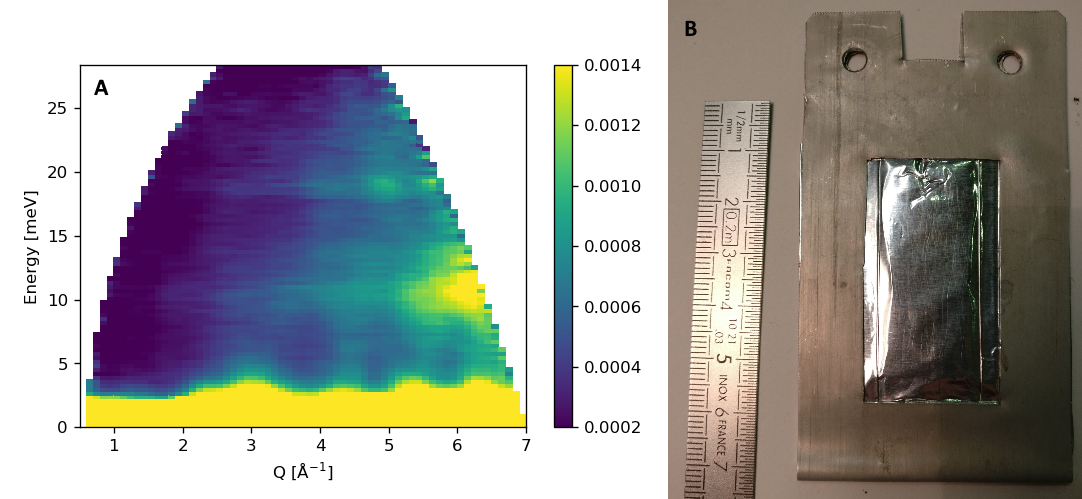
\includegraphics[width=\textwidth]{fig/gdos/sample_sqw.png}
    \caption[$S(\bm{Q}, \omega)$ map and picture of sample]{\textbf{A}: $S(\bm{Q}, \omega)$ map of LSCO3 at \SI{10}{K} with $\lambda = \SI{1.6}{\angstrom}$ incident wavelength. Data has normalized by the Bose factor. \textbf{B:} Sample mounted in cadmium frame.}
    \label{fig:sample_sqw}
\end{figure}

The raw time-of-flight data was reduced to $S(\bm{q},\omega)$ using the \texttt{Mantid} \cite{Arnold2014} software and background was corrected using a sample of polycrystalline vanadium. Due to the isotropic nature of the powder, we only consider the magnitude of $\bm{Q}$ and the resulting data can be viewed in two dimensions as shown in Figure \ref{fig:sample_sqw}A. Obtaining the density-of-states is done in Mantid with the \texttt{ComputeIncoherentDOS} \cite{mantid_dos} algorithm, using the following expression for the one-phonon incoherent scattering function (see section \ref{sec:specific_neutron} for details):

 \[ S^{(1)}_{\mathrm{inc}}(Q,E) = \exp\left(-2\bar{W}(Q)\right) \frac{Q^2}{E} \langle n+\frac{1}{2}\pm\frac{1}{2} \rangle \left[ \sum_k \frac{\sigma_k^{\mathrm{scatt}}}{2m_k} g_k(E) \right]\, , \]
 
 \noindent where $\bar{W} = Q^2 \langle u^2 \rangle / 2$ with $\langle u^2 \rangle$ being the average mean-squared displacement. $n$ is the Bose factor and $E$ is the energy transfer. Finally, the term in brackets is the neutron-weighted density of states with $k$ running over the different elements in our sample. The calculated DOS is given in milibarns/steredians per formula unit per meV. The mean squared displacement is set to $\langle u^2 \rangle = \SI{0.015}{\angstrom\squared}$, which is a good compromise between qualitatively describing our data and the actual values of $\langle u^2 \rangle$ as obtained from experiments \cite{Hafliger2014} and simulations \todo{check these more carefully}.
 
 \begin{table}
    \caption[IN4: $Q$ and $E$ windows for DOS integration]{$Q$ and $E$-ranges used in the computation of DOS. For all spectra a mean squared displacement of $\langle u^2 \rangle = \SI{0.015}{\angstrom\squared}$ was used.}
    \label{tab:qeranges}
    \centering
    \begin{tabular}{llllll}
    \toprule
    $\lambda$ [\AA] & $Q_\text{min}$ [\AA$^{-1}$] & $Q_\text{max}$ [\AA$^{-1}$] & $E_\text{min}$ [meV] & $E_\text{max}$ [meV] & $\Delta E$ [meV] \\ \midrule
    1.6             & 2.0                         & 7.0                         & 4.0                  & 26.0                 & 0.2              \\
    1.1             & 3.0                         & 10.0                        & 7.0                  & 59.0                 & 0.4              \\
    0.85            & 4.0                         & 12.0                        & 15.0                 & 98.0                 & 1.0              \\ \bottomrule
    \end{tabular}
 \end{table}

 In order to get meaningful results from this procedure, reduction of the raw data is usually required. Generally, one chooses a range of $Q$ and $E$ to sum over along with a binning of $E$ (which is measured through time-of-flight and thus on a continuos scale). Since the measured $(Q, E)$ space is different between incident energies, the integration  ranges are chosen for each of the three configurations independently (see Table \ref{tab:in4_mono}). The parameters used for our data reduction are shown in Table \ref{tab:qeranges}.
 
\section{Results}
In order to visualize our spectra, we start by stitching the different wavelengths together. Since the energy resolution of the instrument worsens with increasing incoming energy $E_i$ we stitch together data from the different wavelengths, such that the $\lambda = \SI{1.6}{\angstrom}$ data describes low energies up to $\approx \SI{24}{\milli\eV}$, $\lambda = \SI{1.1}{\angstrom}$ data describes intermediate energies up to $\approx \SI{43}{\milli\eV}$ and $\lambda = \SI{0.85}{\angstrom}$ data describes high energy data.

\begin{figure}
    \centering
    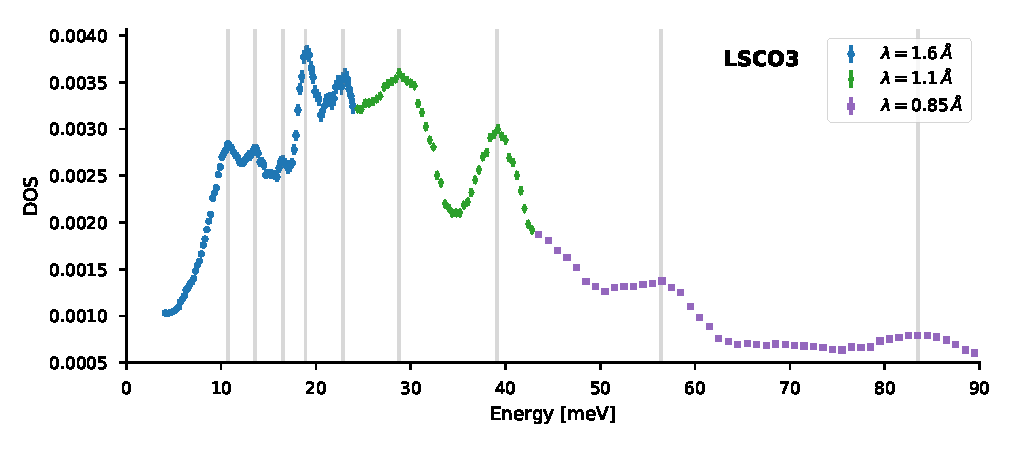
\includegraphics[width=\textwidth]{fig/gdos/in4_lsco3_10k.pdf}
    \caption[gDOS of LSCO3 at 10K. Visualize stitching of data.]{Visualization of the data `stitching' procedure. Our spectra are obtained at low temperatures and we thus only consider neutron energy loss, meaning that the maximal energy of the spectrum is limited by the incoming neutron energy. For this reason, a full spectrum is obtained from three separate measurements and are put together as shown. The energies where data is stitched together is determined by a visual inspection such that we minimize artifacts created by this procedure.}
    \label{fig:in4_stitch}
\end{figure}

Data is stitched together by choosing some cut-off energies such that no features are introduced when we combine the data. The data for $\lambda = \SI{1.1}{\angstrom}$ and $\lambda = \SI{0.85}{\angstrom}$ is then scaled such that we get a continuous spectrum across the full range. For this reason, the absolute values of the DOS is only representative for the $\lambda = \SI{1.6}{\angstrom}$ data. Figure \ref{fig:in4_stitch} shows the result of such a concatenation of data. In addition, vertical lines have been added to show qualitative `peak' features of the spectrum.

\begin{figure}
    \centering
    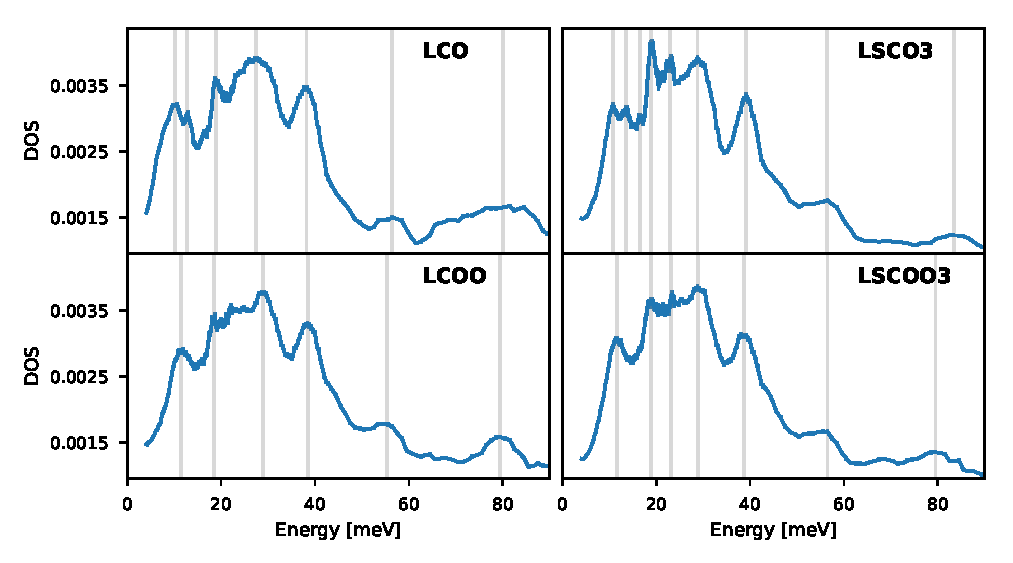
\includegraphics[width=\textwidth]{fig/gdos/in4_10K.pdf}
    \caption[gDOS at \SI{10}{\kelvin}]{DOS of all measured samples (see table \ref{tab:in4_samples} for naming scheme) at \SI{10}{\kelvin}. Data was reduced with Mantid and stitched together from several measurements as described in the text.}
    \label{fig:gdos_10k}
\end{figure}

Applying this procedure to all 4 samples, figure \ref{fig:gdos_10k} shows the phonon DOS for all samples at \SI{10}{\kelvin}. Since no noticeable temperature dependance was found, apart from a tendency to smooth out features, spectra at \SI{60}{\kelvin} and \SI{300}{\kelvin} are not shown here, but can be found in appendix \ref{app:pdos_plots}. Vertical lines in the plots mark peaked features in the spectra and are obtained from a visual inspection. These features are mainly a convenient way to quantify certain differences between samples.

\begin{table}
    \caption{Peaks in the phonon DOS at \SI{10}{\kelvin} of samples considered in this chapter, obtained through visual inspection of figure \ref{fig:gdos_10k} (grey vertical lines).}
    \label{tab:gdos_features_10K}
    \centering
    \begin{tabular}{llllllllll}
        \toprule
          Sample &  $E_1$ & $E_2$ & $E_3$ &  $E_4$ & $E_5$ &  $E_6$ &  $E_7$ &  $E_8$ &  $E_9$ \\
        \midrule
             LCO &   10.2 &  12.8 &     - &   18.9 &     - &   27.5 &   38.2 &   56.4 &   80.0 \\
            LCOO &   11.5 &     - &     - &   18.4 &     - &   28.9 &   38.5 &   55.4 &   79.5 \\
           LSCO3 &   10.7 &  13.6 &  16.5 &   18.9 &  22.9 &   28.8 &   39.1 &   56.4 &   83.5 \\
         LSCO3+O &   11.6 &     - &     - &   18.8 &  23.2 &   28.9 &   38.8 &   56.5 &   79.5 \\
        \bottomrule
    \end{tabular}
\end{table}

Table \ref{tab:gdos_features_10K} shows these features in a list of peak-energies $E_k$, indicating that we can generally identify four separate high-energy peaks at $\approx$ \SIlist{28;39;56;80}{\milli\eV} which are general similar between our samples. Comparison with figure \ref{fig:neutron_bands_dos_lto_afm} shows that these features are qualitatively consistent with the calculated spectrum and that the two high-energy features originate from distinct bands. Features below \SI{30}{\milli\eV} are much more subtle and will have to be analyzed based on changes in the shape of our measured DOS.

Comparing between samples with and without interstitial oxygen, our visual inspection reveals two distinct features. First, we see a subtle modification of the high-energy mode at $\approx \SI{80}{\milli\eV}$, where it seems that spectral weight is moved to lower energies. This is consistent with softening of the Cu-O bond-stretching mode which we will return to in the next chapter. Second, there is a general smoothing of features below \SI{30}{\milli\eV} when introducing interstitial oxygen into the sample. Intuitively, one would expect a smoother DOS with increased disorder, so this observation is, at least qualitatively, consistent with what we would expect. On the other hand, we also see a slight sharpening of features when comparing Sr-doped LSCO3 with the parent compound LCO, inconsistent with the intuitive notion of disorder-induced smoothing of the spectra. LCO, in addition, has a peculiar broad feature at high energies (\SIrange{65}{85}{\milli\eV}), that is unique to that sample and cannot be explained by the logic we used so far.

\section{Comparison with Simulation}
Since the high energy features are either very similar between samples (\SIlist{28;39;56}{\milli\eV}) or considered separately in the next chapter (\SI{80}{\milli\eV}), the following analysis will be focussed on the low-energy part of the phonon DOS. Since the differences between spectra are quite subtle, we consider the effects of oxygen-doping of LSCO3 first, since we are free of the peculiar features of the LCO sample.

\begin{figure}
    \centering
    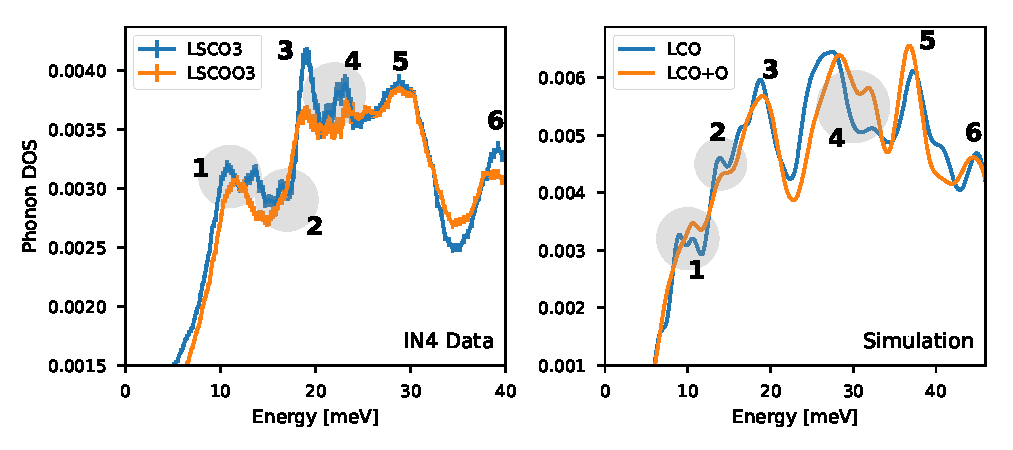
\includegraphics[width=\textwidth]{fig/gdos/simulation_in4_compare.pdf}
    \caption[compare gdos simulation]{\textbf{Left:} Phonon DOS data for LSCO3 and LSCOO3 at \SI{10}{\kelvin}. Features are numbered and dissimilarities between the samples are highlighted \textbf{Right}: Simulations from LCO AFM and LCO+O AFM (see chapter \ref{ch:md} for details) with the same highlighted features as from the data. The simulation data is smoothed by a width that depends on the energy such that $\text{FWHM} = 1.4 + 0.024E$, with $E$ being the energy in \SI{}{\milli\eV}.}
    \label{fig:compare_gdos_sim}
\end{figure}

Figure \ref{fig:compare_gdos_sim} shows a comparison of LSCO3 and LSCOO3 in the low-energy regime below \SI{40}{\milli\eV} alongside a comparison of phonon DOS obtained by molecular dynamics for LCO and LCO+O. Since the Sr content is very low in this sample ($x=0.03$), it is reasonable to assume that it is, at least, approximately similar to LCO with $x=0$. While we had reasonable success in chapter \ref{ch:lowen} when comparing band structures directly, the correspondence between spectra are not quite as convincing in this case. We recover general features as shown in the figure, but the spectral weight and absolute energies deviate slightly from the experimental spectrum (notice the different energy-axes between experiment and simulation).

While the agreement is not perfect, we can still assign the features with some confidence as shown in the labeled features in figure \ref{fig:compare_gdos_sim}. In both the experiment and simulation we see the double-peak at \textbf{(1)} merging, the peak at \textbf{(2)} disappearing and a modification of spectral weight to higher energies at \textbf{(4)} when adding oxygen to the sample. Features at \textbf{(3)}, \textbf{(5)} and \textbf{(6)} stay roughly the same.

\begin{figure}
    \centering
    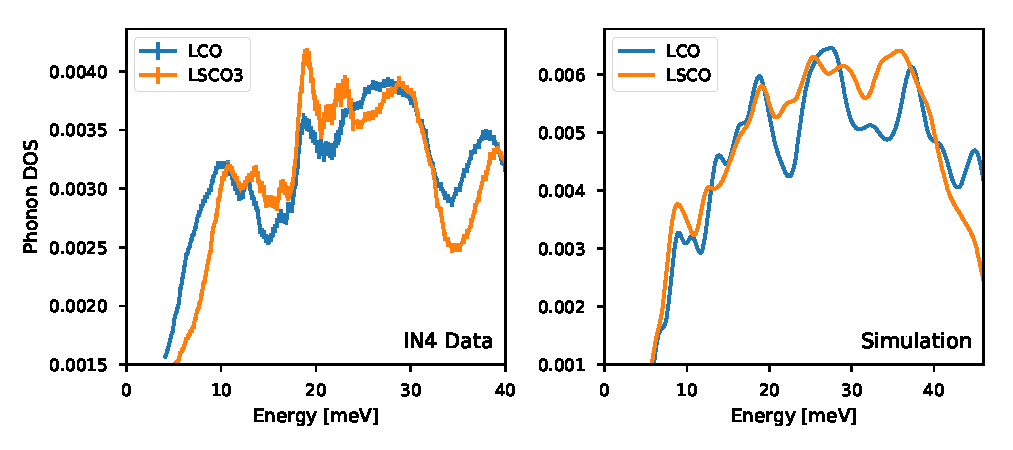
\includegraphics[width=\textwidth]{fig/gdos/lco_lsco_sim_compare.pdf}
    \caption{\textbf{Left:} Phonon DOS data for LCO and LSCO3 at \SI{10}{\kelvin}. \textbf{Right}: Simulations from LCO AFM and LCO+Sr AFM (see chapter \ref{ch:md} for details). The simulation data is smoothed by a width that depends on the energy such that $\text{FWHM} = 1.4 + 0.024E$, with $E$ being the energy in \SI{}{\milli\eV}.}
    \label{fig:compare_lco_lsco_sim}
\end{figure}

Figure \ref{fig:compare_lco_lsco_sim} shows the same idea, but this time for the effect of Sr-doping. We note here that the simulation has roughly twice the doping ($x=0.0625$) of the experimental sample ($x=0.3$), so we cannot expect excellent agreement here. It appears as if the addition of strontium has a similar effect to that of oxygen, but with a smaller magnitude -- there is an overall smoothing of the spectrum due to the introduction of disorder. Interestingly, we reproduce the `dip' at $\approx \SI{30}{\milli\eV}$ in our simulation.

\begin{figure}
    \centering
    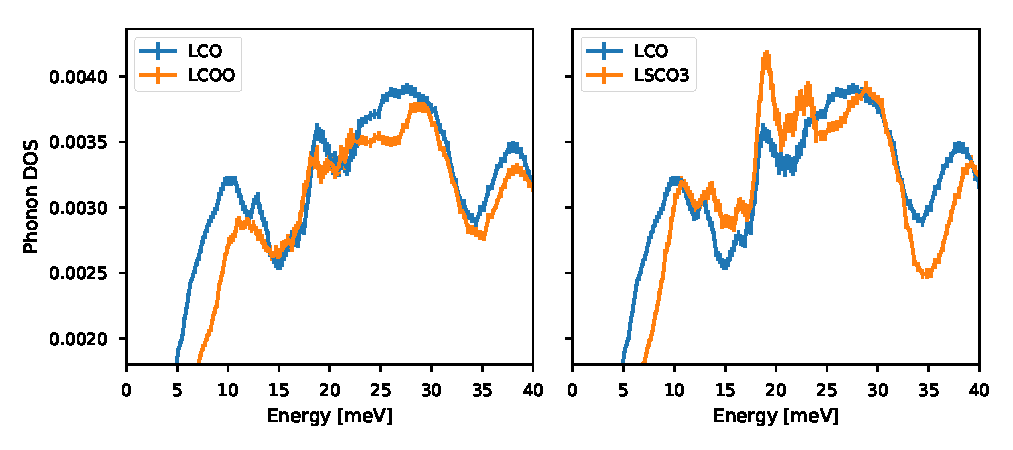
\includegraphics[width=\textwidth]{fig/gdos/in4_low_energy_compare.pdf}
    \caption{Dopant dependence of phonon DOS. \textbf{Left:} Effect of oxygen through a comparison of LCO and LCOO. Notice in particular the modification at low energies. \textbf{Right}: Effect of strontium through a comparison of LCO and LSCO3. While the LSCO3 spectra is much sharper, low energy features are similar in energy when compared to the effect of oxygen.}
    \label{fig:in4_low_energy_compare}
\end{figure}

For the sake of completeness, figure \ref{fig:in4_low_energy_compare} shows the experimental phonon DOS as a function of the two dopants (oxygen, strontium), where it becomes clear that the modification of spectral weight at low energies ($\approx$ \SIrange{5}{15}{\milli\eV}) are more dramatic in the case of oxygen. A corresponding comparison of the simulations can be found in figure \ref{fig:lto_md_defect_comparison}, chapter \ref{ch:md}.

\section{Summary and Discussion}
In this chapter we measured several samples of La$_2$CuO$_4$ with different dopant species in order to shed light on the effect of specific types of chemical disorder on the phonon density of states. While it is possible to discern certain features in the experimental spectra related to the dopant species, differences are in general quite subtle.

With that in mind, we have been able to identify features at low energies which are qualitatively reproduced by our molecular dynamics simulations. At higher energies we only see a modification of the topmost phonon band which will be discussed in the following chapter.

It thus appears as if, despite the significantly reduced simulation precision, that our molecular dynamics simulations can be used to identify a microscopic origin of the modified phonon DOS. The analysis of molecular dynamics simulations concluded that the inclusion of interstitial oxygen species resulted in local `LTT-like tilts' despite the structure being LTO. In fact, it is quite remarkable\todo{is it?} that the structure of these samples are almost identical in our diffraction experiments (the data in chapter \ref{ch:local} is from the same samples), but we clearly see a signature of the dopant species in the dynamics. 

Now, if we believe that our simulations can completely reproduce the peculiarities of the phonon density in these systems,we are also forced to conclude that any differences cannot be directly due to superconductivity. That does not, however, rule out a scenario where these mechanisms are important for superconductivity. As a preliminary outlook, it could be interesting to perform the same measurements on, for example, La$_{1.85}$Sr$_{0.15}$CuO$_4$ ($T_\text{c} = \SI{39}{\kelvin}$) \cite{Radaelli1994a}, La$_{1.48}$Nd$_{0.4}$Sr$_{0.12}$CuO$_4$ (insulating) \cite{Tranquada1995} and La$_{1.875}$Ba$_{0.125}$CuO$_4$ ($T_\text{c} = \SI{4}{\kelvin}$) \cite{Hucker2011} with similar levels of doping but different $T_\text{c}$ and dopant distributions.
